%%%%%%%%%%%%%%%%%%%%%%%%%%%%%%%%%%%%%%%%%%%%%%%%%%%%%%%%%%%%%%%%%%%%%%%%%%%%%%%%%%%%%%%%%
%%%%%%%%%%%%%%%%%%%%%%%%%%%%%%%%%%%%%%%%%%%%%%%%%%%%%%%%%%%%%%%%%%%%%%%%%%%%%%%%%%%%%%%%%
\section{Markov chain Monte Carlo method \mcmc}
%%%%%%%%%%%%%%%%%%%%%%%%%%%%%%%%%%%%%%%%%%%%%%%%%%%%%%%%%%%%%%%%%%%%%%%%%%%%%%%%%%%%%%%%%

The Metropolis algorithm (\MH) was originally introduced by \cite{metropolis1953} for computing properties of substances
composed of interacting individual molecules (when a symmetric proposal is used).
This algorithm has been used extensively in statistical physics.
A generalization to non-symmetric proposals was introduced by \cite{hastings70}.

The Metropolis algorithm or one of the variants, are often used in situations where the \apriori\ knowledge of the target distribution is quite limited.

The drawback of \mcmc\ is that the acceptance rate is generally very
low due to the large dimensionality of the stochastic fields.
Thus, \mcmc\ simulations usually require thousands of iterations before converging to a steady state. Each iteration involves the computation of the fine-scale flow problem which is very
CPU demanding. This makes \mcmc\ simulations very expensive from the computational point of view. In order to overcome this difficulty, we have introduced multi-stage, multi-physics \mcmc\
methods \citep{ginting11,ginting12,ginting13d}.
The shape and size of the proposal distribution $\propf{\cdot}$ is known to be very crucial for the convergence of the Markov chain corresponding the \mcmc\ algorithm \citep{haario99}.

Several methods have been developed in order to speed up the convergence: Adaptive Proposal (\AP) \citep{haario99}; Adaptive Metropolis (\AM) \citep{haario2001}; Delayed Rejection (\DR) \citep{Tierney1994,TierneyMira1999}; Delayed Rejection Adaptive Metropolis algorithm (\DRAM) \citep{Haario2006}; Single Component Adaptive Metropolis (\SCAM) \citep{haario2005}; Differential Evolution  Markov Chain (\DE) \citep{vrugt2003,terbraak2006}; DiffeRential Evolution Adaptive Metropolis (\DREAM) \citep{vrugt2008}, among others.

%%%%%%%%%%%%%%%%%%%%%%%%%%%%%%%%%%%%%%%%%%%%%%%%%%%%%%%%%%%%%%%%%%
\subsection{Differential Evolution Metropolis (\DE)}
%%%%%%%%%%%%%%%%%%%%%%%%%%%%%%%%%%%%%%%%%%%%%%%%%%%%%%%%%%%%%%%%%%

In this paper we choose the Differential Evolution Metropolis (\DE) to perform our experiments.
\DE\ is a population \mcmc\ algorithm, in which multiple chains are run in parallel.
The jumps are simply a fixed multiple of the differences of two random parameter vectors that are currently in the population.

\cite{vrugt2003} developed a population-based \mcmc\ algorithm to enhance the efficiency of \mcmc\ sampling integrating Differential Evolution genetic algorithm ideas to Metropolis algoritm, resulting in the Differential Evolution Markov chain Monte Carlo method (\DE) that allows for the exchange of information among multiple chains running in parallel.
According to \cite{vrugt2003,braak2006}, this choice yields an appropriate scale and orientation for the jumping distribution.

Consider the $\nc$, $\dim$-dimensional, parameters $\staten{t}_{i}$, $i=1,2,\dots,\nc$, members of population $\mat{X}^{(t)}$ at state $t$.
Thus, $\mat{X}^{(t)}$ is a $\nc \times \dim$ matrix.
To draw the samples and to ensure that the whole parameter space can be reached we consider

\begin{equation}
 \state = \staten{t}_{r_1} + \scfde\left( \staten{t}_{r_2}-\staten{t}_{r_3} \right) + \vet{e},
 \label{proposalDE}
\end{equation}

\noindent where $\vet{e}$ is drawn from a symmetric distribution with a small variance compared to that of the target, but with
unbounded support, e.g. $\vet{e}\sim\normalf{\vet{0}}{b\mat{I}_{\dim}}$ with $b$ small.
Here, $\staten{t}_{r_2}$ and $\staten{t}_{r_2}$ are randomly selected without replacement from the population current $\mat{X}^{(t)}$ (the population without $\staten{t}_{r_1}$), i.e. $r_{1} \neq r_{2} \neq r_{3}$.

For large $\nc$ and small $b$, the proposal \eqp{proposalDE} thus looks like $\state = \staten{t} + \scfde \varepsilon$ with
$\mean{\varepsilon}=\vet{0}$ and $\cov{\varepsilon} = 2\covs$, the covariance matrix of the target.
In particular, if $\post{\cdot}$ is multivariate normal, then $\scfde\varepsilon\sim\normalf{\vet{0}}{2\scfde^2\covs}$ so that \DE\
is expected to behave like \RW. From the guidelines for $\scf$ in \citep{roberts2001} the optimal choice of $\scfde$ is then $2.38 / \sqrt{2\dim}$.
This choice of $\scfde$ is expected to give an acceptance probability of $0.44$ for $\dim = 1$, $0.28$ for $\dim = 5$ and $0.23$ for large $\dim$.
If the initial population is drawn from the prior, \DE\ translates the ``prior population'' to the ``posterior population''.

%%%%%%%%%%%%%%%%%%%%%%%%%%%%%%%%%%%%%%%%%%%%%%%%%%%%%%%%%%%%%%%%%%
\subsubsection{Autoregressive Differential Evolution Metropolis}
%%%%%%%%%%%%%%%%%%%%%%%%%%%%%%%%%%%%%%%%%%%%%%%%%%%%%%%%%%%%%%%%%%

Consider a set of high dimensional ($\dim \gg 1$) random vectors $\staten{t}_{i}$, $i=1,\dots,\nc$ independent and identically distributed.
More specifically, $\staten{t}_{i}\sim\normalf{\vet{0}}{\vari{\staten{t}}\mat{I}_{\dim}},\quad \forall i$.
In other words, $\staten{t}_{i}$ are independent standard Gaussian random variables.
Using \eqp{proposalDE} to yield the new generation (proposals) and considering that $\vari{\vet{e}}$ is negligible, the variance of $\state$ is given by:

\begin{equation}
 \begin{array}{rcl}
  \vari{\state} & = & \vari{\staten{t}_{r_1}} + \scfde^{2}\left( \vari{\staten{t}_{r_2}} + \vari{\staten{t}_{r_3}} \right)\\ \\
                & = & \vari{\staten{t}} \left( 1 + 2 \scfde^{2} \right).
 \end{array}
 \label{eq:var}
\end{equation}

\noindent The previous result of \eq{eq:var} shows that as the iterations $t$ evolve, there is a progressive increase in the variance of the new proposals, which can cause problems in the convergence of the method.
To overcome this problem, we propose a modification of \DE\ sampler \eqp{proposalDE} inspired by the autoregressive version of \RW\ (\eq{eq:autorw}):

\begin{equation}
 \state = \left( \sqrt{1 - 2 \scfde^2} \right) \staten{t}_{r_1} + \scfde\left( \staten{t}_{r_2}-\staten{t}_{r_3} \right) + \vet{e},
 \label{proposalARDE}
\end{equation}
\noindent with the following restriction: $\scfde = \min\left(2.38 / \sqrt{2\dim}, \sqrt{1/2} \right)$.
In order words, the minimal dimension is $6$ ($\dim \geqslant 6$).
The proposal \eq{proposalARDE} ensures that $\vari{\state} = \vari{\staten{t}},\quad \forall i$.
The variation of $\scfde(\dim)$ and $f(\dim) = \sqrt{1 - 2\left(\dfrac{2.38}{\sqrt{\dim}}\right)^2}$ are shown in \fig{ArJumpDE}.
Again, this method is recommended for high-dimensional problems.

\begin{figure}[H]
 \centering
 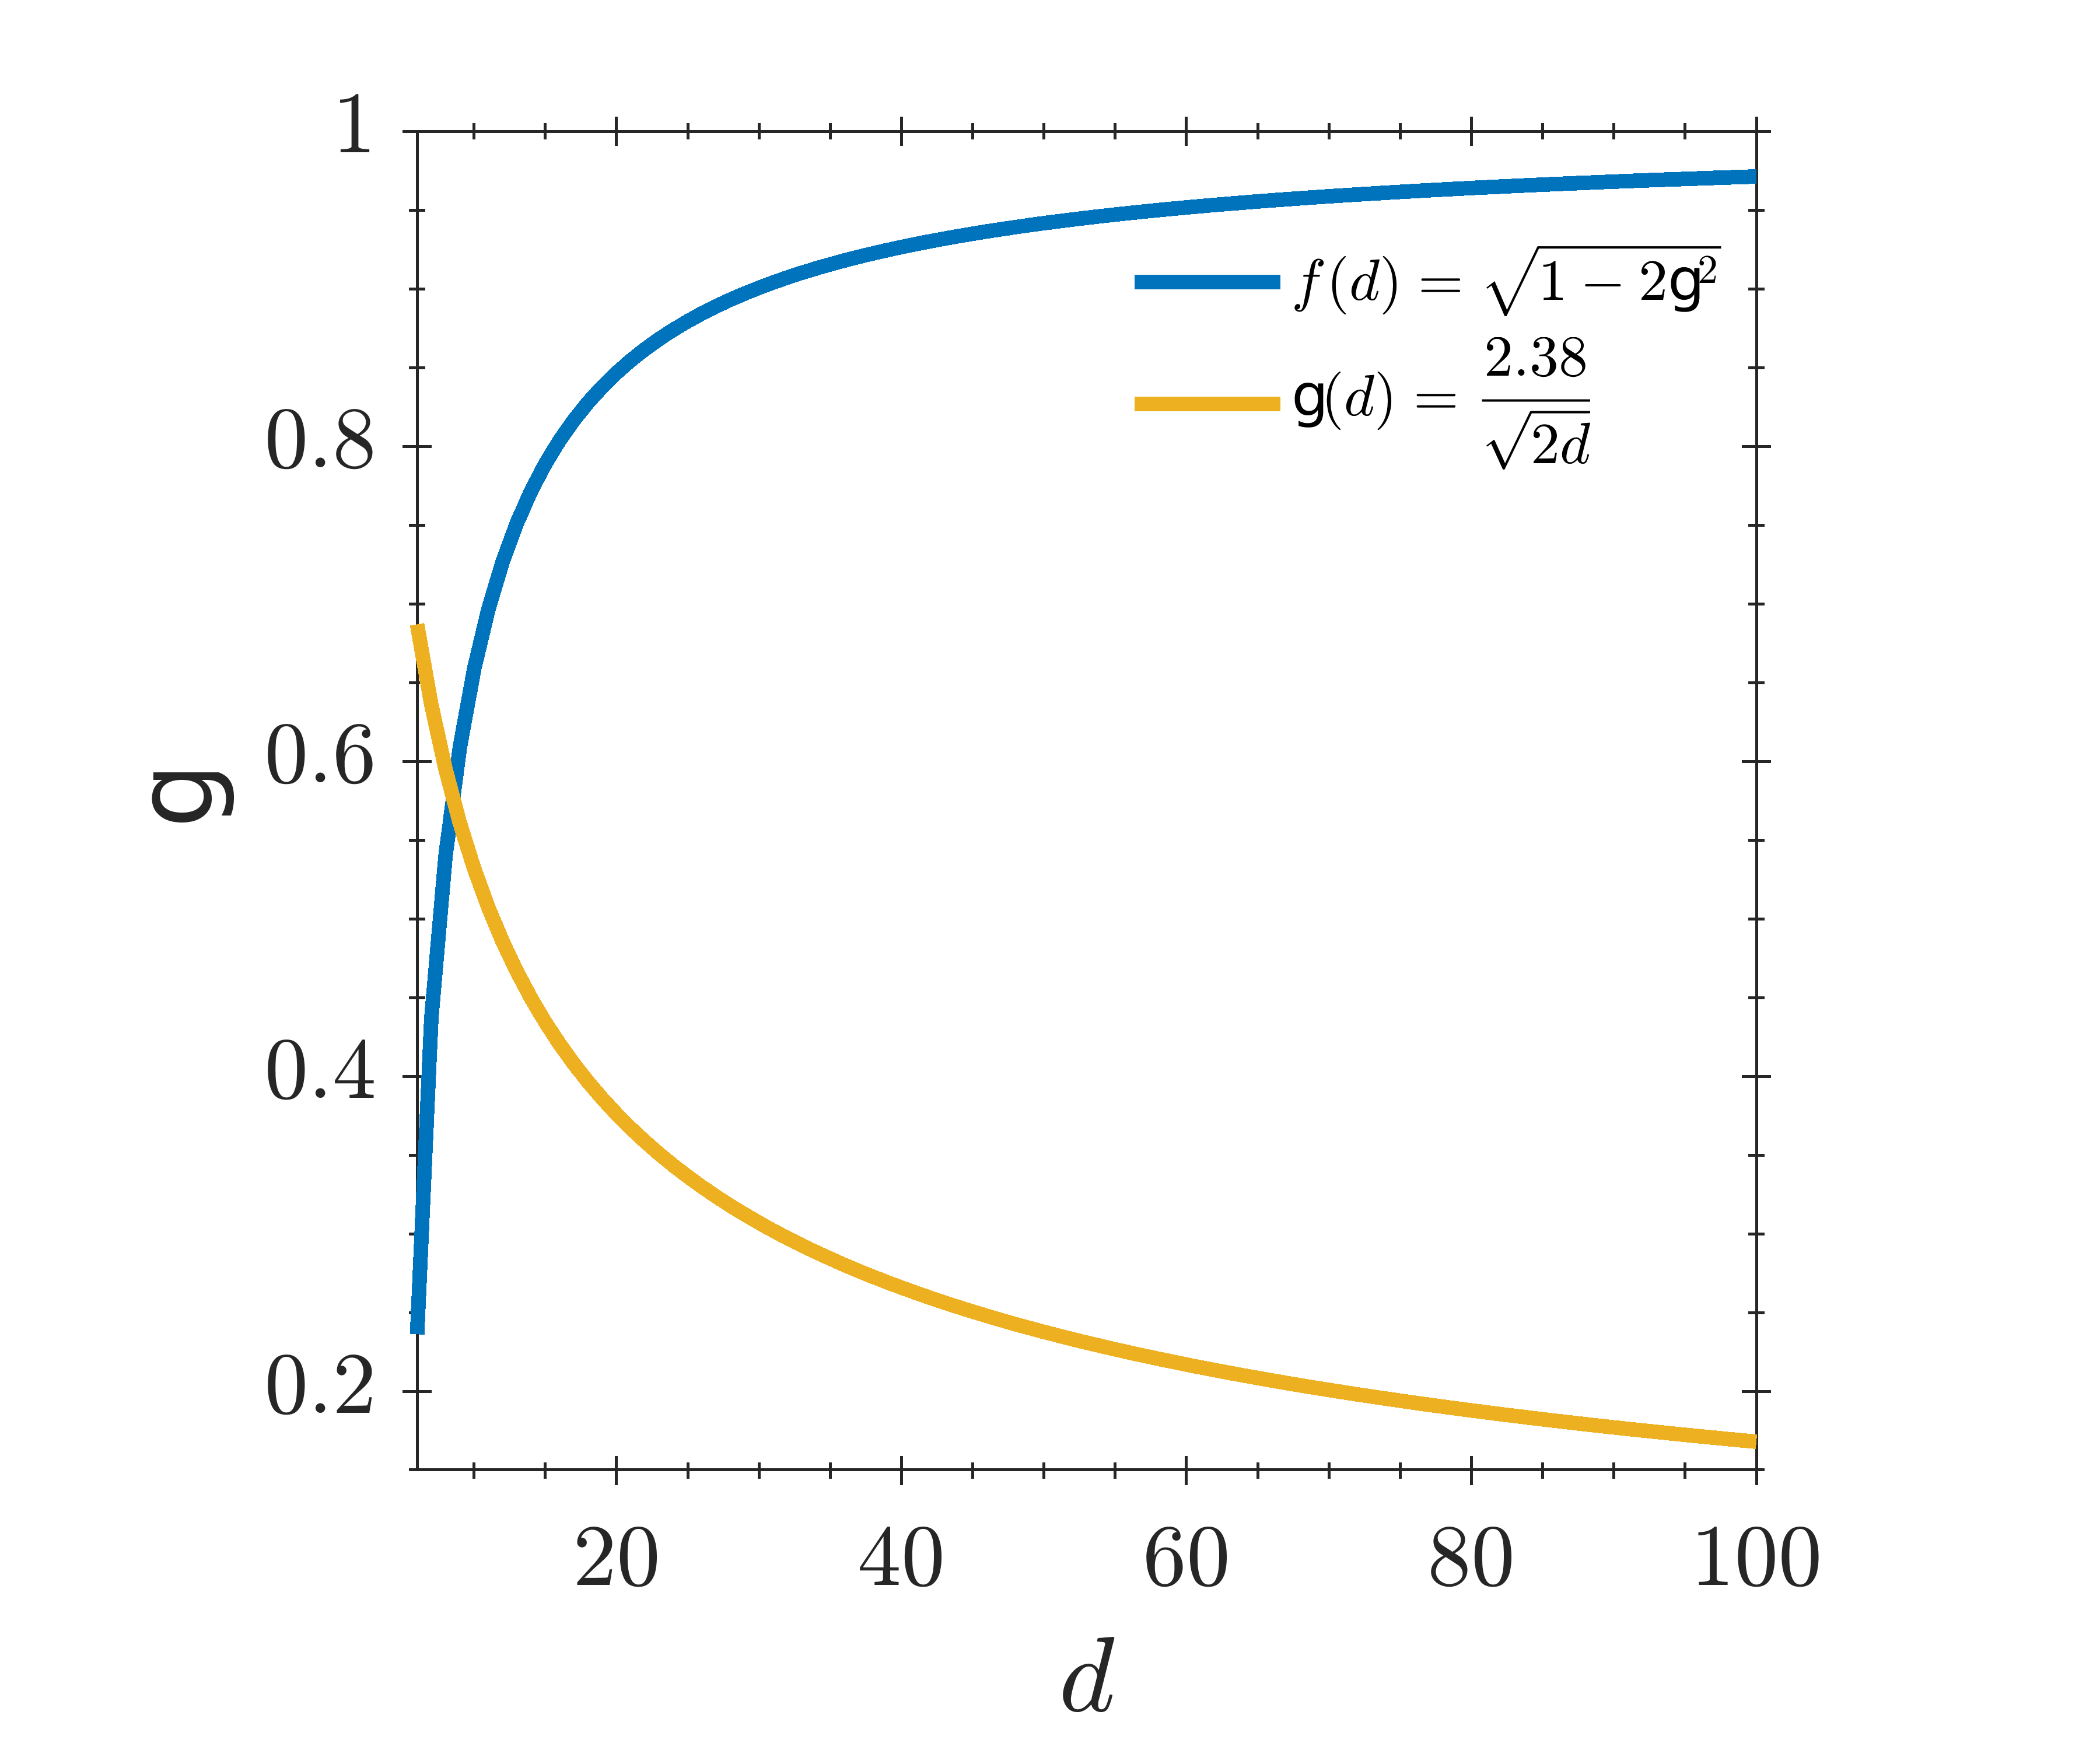
\includegraphics[scale=0.5]{./figuras/Jumps_DE.png}
 \caption{Coefficeents associated with autoregressive jump for autoregressive \DE.}
 \label{ArJumpDE}
\end{figure}

%%%%%%%%%%%%%%%%%%%%%%%%%%%%%%%%%%%%%%%%%%%%%%%%%%%%%%%%%%%%%%%%%%
%%%%%%%%%%%%%%%%%%%%%%%%%%%%%%%%%%%%%%%%%%%%%%%%%%%%%%%%%%%%%%%%%%
\subsection{Dimensionality reduction}
%%%%%%%%%%%%%%%%%%%%%%%%%%%%%%%%%%%%%%%%%%%%%%%%%%%%%%%%%%%%%%%%%%

Another technique that has been widely used to speed up the convergence in the \mcmc\ framework is the reduction of the stochastic dimension using the \KL\ (\kl) expansion
\citep{efendiev05,efendiev2006,das10,mondal10,ginting11,ginting12}.
The subsurface stochastic field (permeability, porosity, Young's modulus, etc.) may be represented as a series expansion
involving a complete set of deterministic functions with correspondent random coefficients using the \kl\ expansion, proposed independently by \cite{karhunen46} and \cite{loeve55}, which is based on the eigen-decomposition of the covariance function.
If the eigenvalues decay very fast for a specific covariance function, only a small number of terms need to be retained in the truncated expansion.
This procedure allows us to perform the search in a smaller parameter space.

